\section{Comparision}\label{sec:Comparision}

\subsection{Ballistic Deployment}

\begin{figure} \centering
  {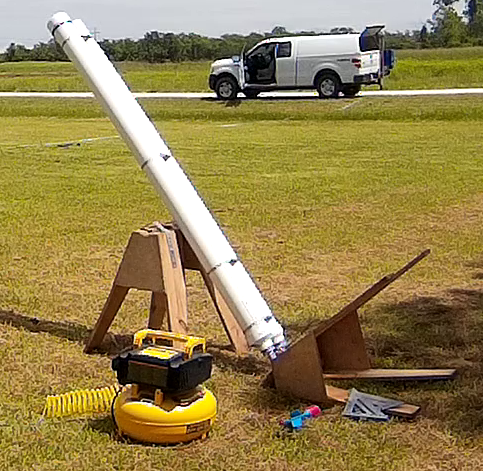
\includegraphics[width=\columnwidth]{PotatoCannon.png}}
 \caption{A pneumatic launcher for SeismicDarts.  Ballistic dart deployment has limited usefulness because the incident angle is equal to the firing angle.} 
 \label{fig:TradvsAutoDrop}
\end{figure}



\subsection{Simulation Studies}

A scheduling system to compare  time and costs for seismic surveys with varying numbers of Deployment Units, SeismicSpiders, SmartDarts, and Human manual laborers was coded in  {\sc Matlab}, available at \cite{Srikanth2016seismicScheduler}.

This tool allows us to examine engineering and logistic tradeoffs quickly in simulation.  For example, Fig.~\ref{fig:DronevsTime} assumes a fixed number of darts (5000), and examines the finishing time with 5 to 500 UAVs.  The time required decays asymptotically, but  XX drones requires only 5\% more time than 5000 drones, indicating that XX are sufficient for the task. Lines are also plotted for XX,XX, and XX total darts.  In each case, substantial cost savings can be obtained by selecting the number of drones required to complete within 5\% of the optimal time.
The tool is useful for comparing the effectiveness of heterogeneous teams.  Table XX compares surveying a 1 km x 10 km strip of land with team (a) XX drones, (b) XX SeismicSpiders and XX drones, (c) XX humans.  Team (a) completed XX times faster than team (c).

\begin{figure*}
\centering
\renewcommand{\figwid}{0.5\columnwidth}
\begin{overpic}[width =\figwid]{sim1_1.pdf}
\end{overpic}
\begin{overpic}[width =\figwid]{sim1_2.pdf}
\end{overpic}
\begin{overpic}[width =\figwid]{sim1_3.pdf}
\end{overpic}
\begin{overpic}[width =\figwid]{sim1_4.pdf}
\end{overpic}

\caption{Simulations were performed to estimate time take by different sensors a.) Only seismic spiders b.) Smart darts and deployment system c.) Heterogeneous System d.) Human workers
\label{fig:Sim_overview}}
\end{figure*}
\begin{figure} \centering
  {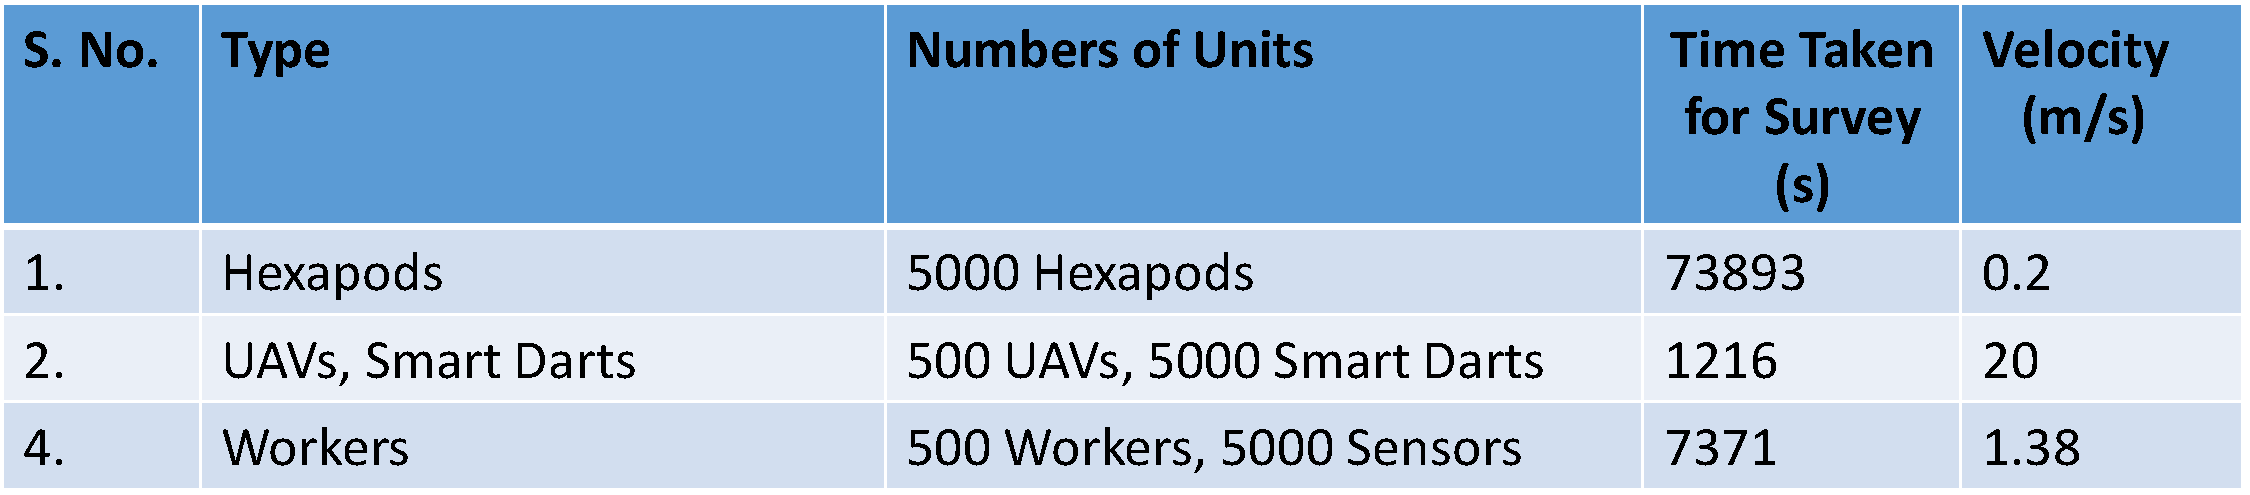
\includegraphics[width=\columnwidth]{simulation_table.pdf}}
 \caption{Simulations were performed to estimate time take by different sensors a.) Only seismic spiders b.) Smart darts and deployment system c.) Heterogeneous System d.) Human workers} 
 \label{fig:TradvsAutoDrop}
\end{figure}
\begin{figure} \centering
  {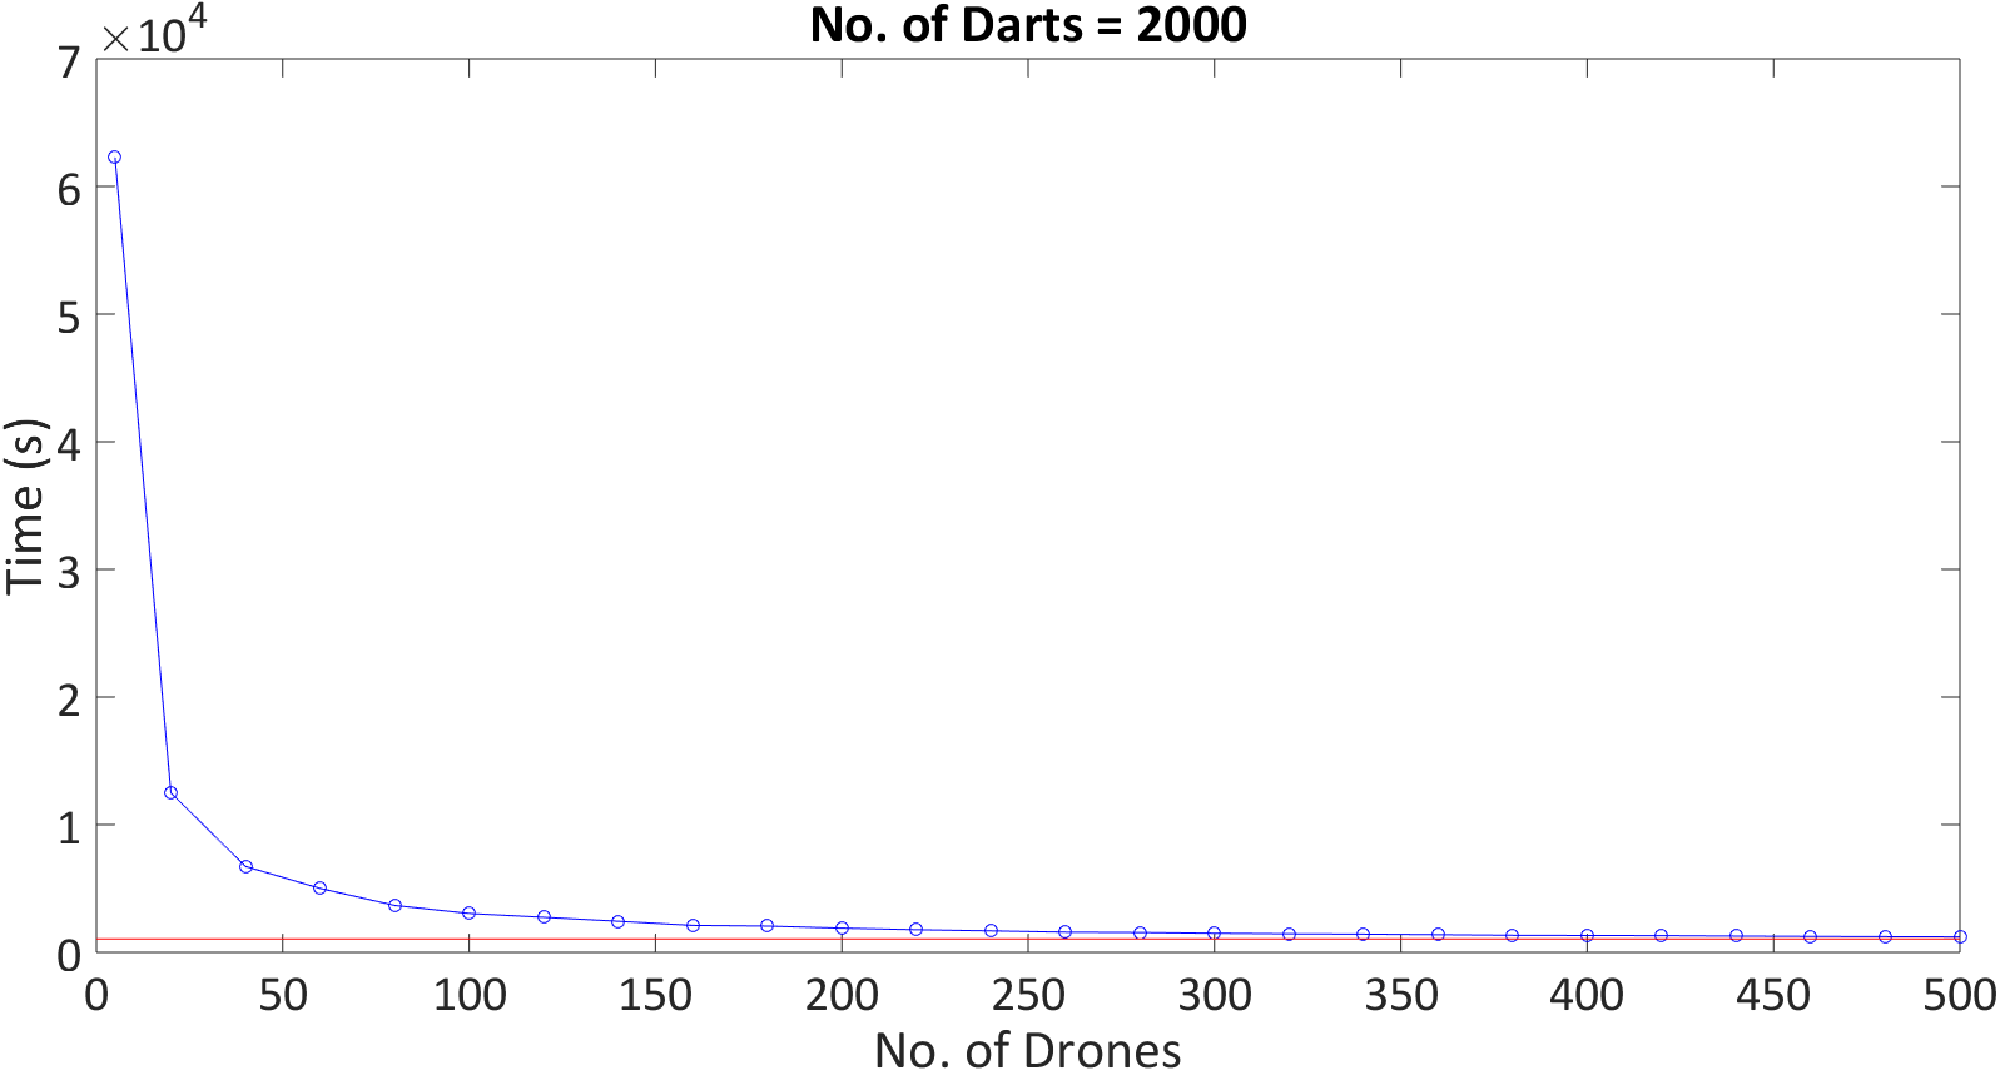
\includegraphics[width=\columnwidth]{DronevsTime.pdf}}
 \caption{This plot captures no. of drones vs time taken.} 
 \label{fig:DronevsTime}
\end{figure}
\begin{figure} \centering
  {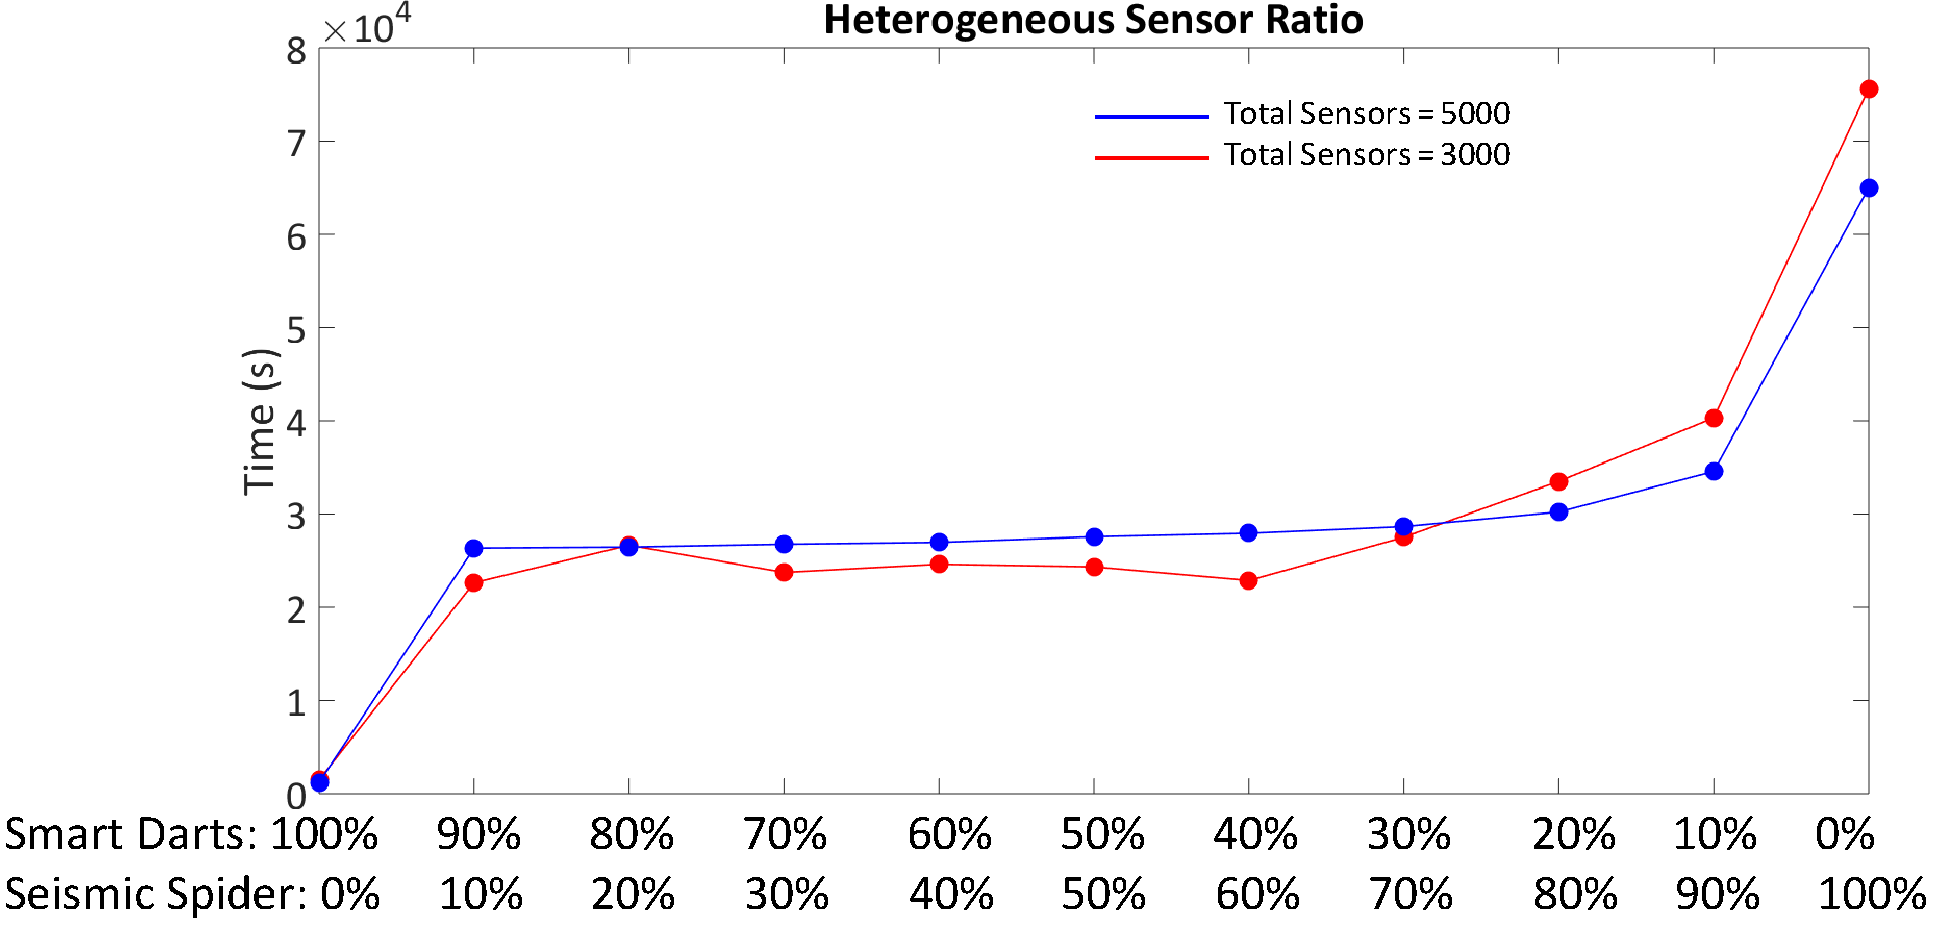
\includegraphics[width=\columnwidth]{het_sen_ratio.pdf}}
 \caption{This plot captures time with respect to different sensor ratios. The total number of sensors(5000,3000) were kept constant. UAVs were taken to be 10\% of darts for this experiment. } 
 \label{fig:DronevsTime}
\end{figure}